% Full instructions available at:
% https://github.com/elauksap/focus-beamertheme

\documentclass[9pt]{beamer}
\usetheme{focus}

%%%%%%%%%%%%%%%%%%%%%%%%%%%%%%%%%%%%%%%%%%%%%%%%%%%%%%%%%%%%%%%%%%%%%
% Typography, change document font
\usepackage[tt=false, type1=true]{libertine}
\usepackage[varqu]{zi4}
\usepackage[libertine]{newtxmath}
\usepackage[T1]{fontenc}

\usepackage[protrusion=true,expansion=true]{microtype}

% Disable paragraph indentation, and increase gap
\usepackage{parskip}

%Matrix
\usepackage{tabstackengine}
\setstackEOL{;}% row separator
\setstackTAB{,}% column separator
\setstacktabbedgap{1ex}% inter-column gap 
\setstackgap{L}{1.0\normalbaselineskip}% inter-row baselineskip
\let\mat\bracketMatrixstack

\newcommand{\pth}{Figure/}
\newcommand{\ve}[1]{\mathbf{#1}}

% Copyright (C) 2018-2019 Pasquale Claudio Africa and the LaTeX community.
% A full list of contributors can be found at
%
%     https://github.com/elauksap/focus-beamertheme
% 
% This file is part of beamerthemefocus.
% 
% beamerthemefocus is free software: you can redistribute it and/or modify
% it under the terms of the GNU General Public License as published by
% the Free Software Foundation, either version 3 of the License, or
% (at your option) any later version.
% 
% beamerthemefocus is distributed in the hope that it will be useful,
% but WITHOUT ANY WARRANTY; without even the implied warranty of
% MERCHANTABILITY or FITNESS FOR A PARTICULAR PURPOSE. See the
% GNU General Public License for more details.
% 
% You should have received a copy of the GNU General Public License
% along with beamerthemefocus. If not, see <http://www.gnu.org/licenses/>.

\mode<presentation>


% DEFINE COLORS. ---------------------------------------------------------------
\definecolor{main}{RGB}{134, 161, 174}
\definecolor{main2}{RGB}{104, 131, 144}
\definecolor{textc}{RGB}{20, 20, 20}
\definecolor{background}{RGB}{255, 255, 255}

\definecolor{alert}{RGB}{180, 0, 0}
\definecolor{example}{RGB}{0, 110, 0}


% SET COLORS. ------------------------------------------------------------------
\setbeamercolor{normal text}{fg=textc, bg=background}
\setbeamercolor{alerted text}{fg=textc}
\setbeamercolor{example text}{fg=textc}

\setbeamercolor{titlelike}{fg=background, bg=main}
\setbeamercolor{frametitle}{parent={titlelike}}

\setbeamercolor{footline}{fg=background, bg=main2}

\setbeamercolor{block title}{bg=main!80!background, fg=background}
\setbeamercolor{block body}{bg=main!10!background, fg=textc}

\setbeamercolor{block title alerted}{bg=alert, fg=background}
\setbeamercolor{block body alerted}{bg=alert!10!background, fg=textc}

\setbeamercolor{block title example}{bg=example, fg=background}
\setbeamercolor{block body example}{bg=example!10!background, fg=textc}

\setbeamercolor{itemize item}{fg=textc}
\setbeamercolor{itemize subitem}{fg=textc}

\setbeamercolor{enumerate item}{fg=textc!70!black}
\setbeamercolor{enumerate subitem}{fg=textc!70!black}

\setbeamercolor{description item}{fg=textc!70!black}
\setbeamercolor{description subitem}{fg=textc!70!black}

\setbeamercolor{caption name}{fg=textc}

\setbeamercolor{section in toc}{fg=textc}
\setbeamercolor{subsection in toc}{fg=textc}
\setbeamercolor{section number projected}{bg=textc}
\setbeamercolor{subsection number projected}{bg=textc}

\setbeamercolor{bibliography item}{fg=main}
\setbeamercolor{bibliography entry author}{fg=main!70!black}
\setbeamercolor{bibliography entry title}{fg=main}
\setbeamercolor{bibliography entry location}{fg=main}
\setbeamercolor{bibliography entry note}{fg=main}

\mode<all>


\begin{document}
	\tableofcontents

\section{Stress and equilibrium : \today}

	\begin{frame}
		\begin{itemize}
		\item We are dealing with different configurations. One configuration is maybe unstressed and the deformed one is. So at the deformed x we should get an equilibrium of stresses and the external loads
		\item Now, the actual stresses at the deformed or current configuration is the Cauchy stress : defined as the force in different directions by the area in different planes
		\item Stresses can also be defined with respect to the initial configuration X			
					
		\end{itemize}

	\end{frame}

	\begin{frame}{Cauchy stress tensor}
		\begin{figure}
			\centering
			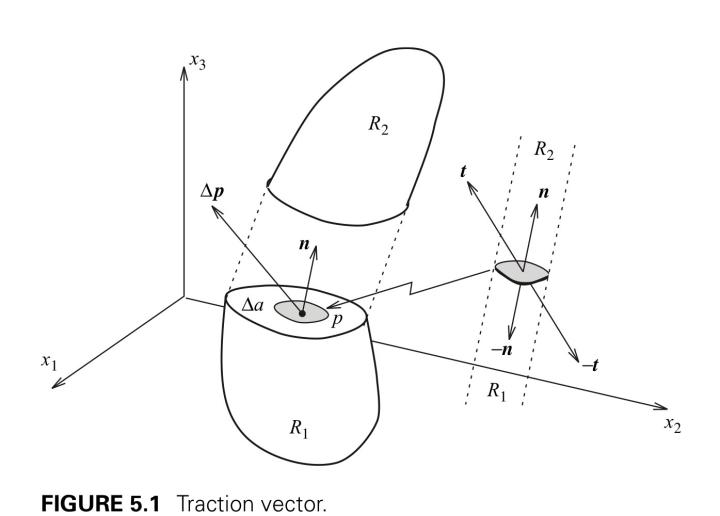
\includegraphics[width=0.5\linewidth]{Figure/fig7}
		\end{figure}
		At the deformed configuration :
		\begin{itemize}
			\item See two bodies $R_1$ and $R_2$ free body with force acting on them
			\item Imagine the traction vector on a small area element : ${t(n) = \frac{\Delta p}{\Delta a}}$ as lim $\Delta a \rightarrow 0$ where $\Delta p$ is the resultant force
			\item Obviously $t$ and $n$ will depend on the surface it acts on. Here on the right we can see that based on the surface we get opposite forces. (In the negative normal , we will get negative force which is positive in that direction!)

		\end{itemize}
	\end{frame}

	\begin{frame}
		\begin{figure}
			\centering
			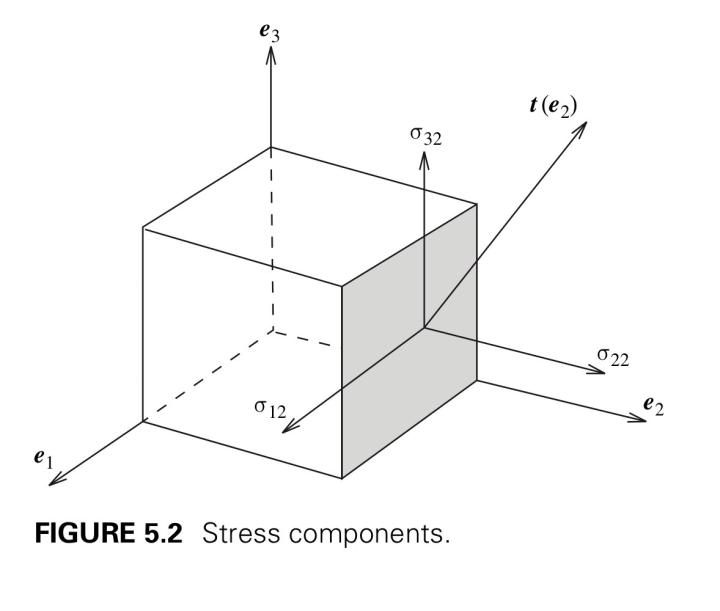
\includegraphics[width=0.5\linewidth]{Figure/fig8}
		\end{figure}
	
		\begin{itemize}
			\item Let us denote the traction acting on the surface having normals denoted by $e_1, e_2,e_3$
			\item Remember in the other slice we will have an opposite reaction
			\begin{equation}
			\begin{aligned}
			\ve{t(e_1) = \sigma_{j1}e_j} \\\ve{t(e_2) = \sigma_{j2}e_j}\\\ve{t(e_3) = \sigma_{j3}e_j}
			\end{aligned}
			\end{equation}
			\item Or $\ve{t_i = \sigma_{ji}e_j}$ or $\ve{t = \sigma^T e}$
		\end{itemize}
	\end{frame}

	\begin{frame}
		\begin{figure}
			\centering
			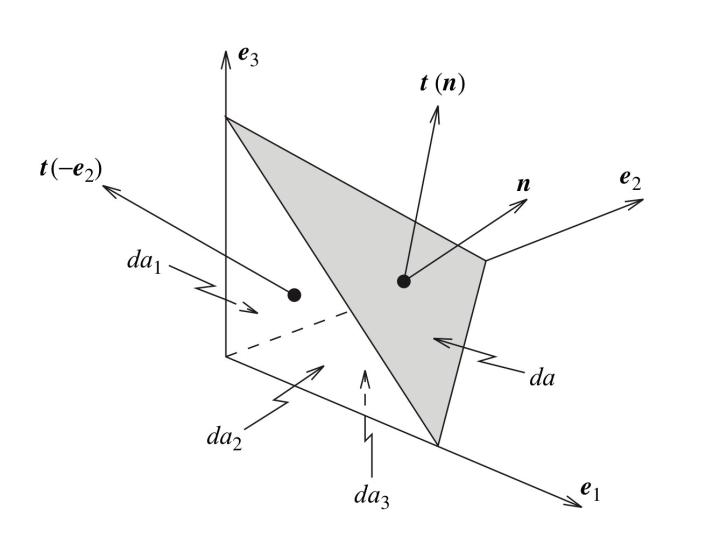
\includegraphics[width=0.5\linewidth]{Figure/fig9}
		\end{figure}
		
		Now let us look if we take a plane cut of that sphere. Again by context of opposite reactions. All the forces should be equal. So we will use here the concept of equilibrium between the traction vector we have defined in the last slide with respect to some basis and the traction vector defined on the angled plane.
		
		\begin{block}{Equilibrium}
			\begin{equation}
			\ve{t(n)}da + t(\ve{-e_i})da_i + \ve{f}dv = 0
			\end{equation}
			This states that the force vector on the inclined cut should be in equilibrium with the opposite forces defined on the negative sufraces and the body force
		\end{block}
	
	\end{frame}

	\begin{frame}
		\begin{itemize}
			\item  Now the areas (Because they are with defined respect to the basis vectors) can be written as the projection of the inclined area
			\begin{equation}
				da_i = da(\ve{n.e_i})
			\end{equation}
			\item Diving by da we get 
			\begin{equation}
			\ve{t(n)} + t(\ve{-e_i})\frac{da(\ve{n.e_i})}{da} + \ve{f}\frac{dv}{da} = 0
			\end{equation}
			\item $\frac{dv}{da} \rightarrow 0$  ( I don't know why????????????????)
			\item We get :
			\begin{equation}
			\begin{aligned}
			\ve{t(n)} = - t(\ve{-e_i})(\ve{n.e_i}) =  t(\ve{e_i})(\ve{n.e_i})\\
			\ve{t(n)} = (\ve{\sigma_{ji}e_j})(\ve{n.e_i}) \\
			\ve{t(n)} = (\ve{\sigma_{ij}e_i})(\ve{n.e_j}) \text{Replacing indexs}\\
			\end{aligned}
			\end{equation}
		\end{itemize}
	\end{frame}


	\begin{frame}
		\begin{itemize}
			\item Very interesting, we started off with a statement that the resultant force on the plane is equal to the summation of the opposite forces
			\item Then we got the traction vector is equal to the traction vectors multiplied by some scalar product (Think of ratio)
			\item $t(\ve{e_i})(\ve{n.e_i})$ states the traction in $e_i$ direction multiplied by the projection of planar area for i =1,2,3
			\item Now we can replace the traction vector by the components of stress vectors in the basis direction $\ve{t(n)} = (\ve{\sigma_{ij}e_i})(\ve{n.e_j})$
			\item Here we have to point out that $\sigma_{ij}$ has not been described as a tensor yet\\		
		\end{itemize}
	\end{frame}

	\begin{frame}{Tensor insight}
		\begin{itemize}
			\item If we look at $\ve{t(n)} = (\sigma_{ij}\ve{e_i})(\ve{n.e_j})$ , we can see that $\sigma_{ij}$ is just a component and $\ve{n.e_j}$ is a scalar (Or a projection).
			\item That scalar value then becomes the component of $e_i$. Lets see what that means 
			\begin{equation}
			\begin{aligned}
			\sigma_{12}\ve{e_1(n.e_2)}= \sigma_{12}\mat{1;0;0}(\mat{n_1,n_2,n_3}\mat{0;1;0}) = \sigma_{12} n_2 \mat{1;0;0}
			\end{aligned}
			\end{equation}
			\item So we took the second component of $n$ and added to the result of linear map in $e_1$.This is what we do when we multiply the first row of a matrix and a vector. We add all the components of the vector to keep in the first component of the output
			\item So we can write it therefore as
			\begin{equation}
				\ve{e_i(n.e_j) = (e_i \otimes e_j).n} 
			\end{equation}
			which states that the tensor takes the projection of $e_j$ in n and maps as components of $e_i$
			\item This then allows us to understand that $\sigma_{ij}(\ve{e_i \otimes e_j})$ is a tensor $\sigma$
		\end{itemize}
	\end{frame}

	\begin{frame}
		\begin{itemize}
			\item In simplicity $\ve{t(n)} = (\sigma_{ij}\ve{e_i})(\ve{n.e_j})$ says that for every cut, $\ve{n}$ 
			\begin{equation}
			\mat{t_1;t_2;t_3} = \mat{\sigma_{11}\ve{e_1(n.e_1)} + \sigma_{12}\ve{e_1(n.e_2)} + \sigma_{13}\ve{e_1(n.e_3)};\sigma_{21}\ve{e_2(n.e_1)} + \sigma_{22}\ve{e_2(n.e_2)} + \sigma_{23}\ve{e_2(n.e_3)} ; \sigma_{31}\ve{e_3(n.e_1)} + \sigma_{32}\ve{e_3(n.e_2)} + \sigma_{33}\ve{e_3(n.e_3)}}
			\end{equation}
			FIXXX. These are not components yet!
			\item And now you can see that $\ve{e_i \otimes e_j}$ just makes the tensor take the right projection and keeps in the component in the output
			\item $\sigma_{ij}n_j$ is therefore something like taking the projection of j for every component i
		\end{itemize}
	\end{frame}

	\begin{frame}{Problem \#1}
		\begin{figure}
			\centering
			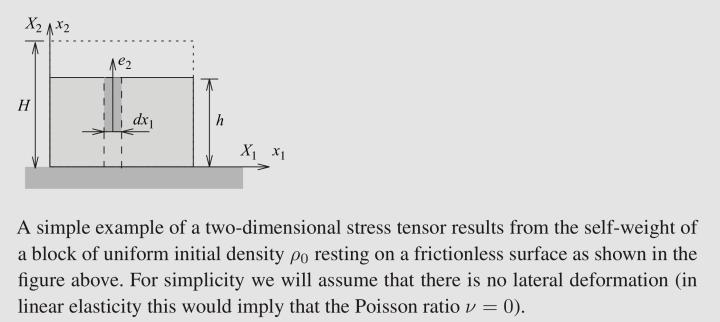
\includegraphics[width=0.7\linewidth]{Figure/fig10}
		\end{figure}
	\begin{itemize}
		\item $t(\ve{e_2}) = \dfrac{\left(-\int_{y}^{h} \rho g dx_2 \right)\ve{e_2}dx_1}{dx_1}$
		\item Mass conservation $\rho dx_1dx_2 = \rho_o dX_1dX_2$ + poisson = 0 give :
		\begin{equation}
		t(\ve{e_2}) = \rho_o g (H- X_2) \ve{e_2}
		\end{equation}
		\begin{equation}
		t(\ve{e_2}) = \sigma_{12}\ve{e_1} + \sigma_{22}\ve{e_2}
		\end{equation}
		so $\sigma_{12} = 0$ , so you can construct $\sigma$. Check Bonet Pge 138
	\end{itemize}
	\end{frame}

	\begin{frame}{Principal basis}
		\begin{itemize}
			\item Obviously the Cauchy stress components can be described with respect to its principal directions $\phi_1,\phi_2,\phi_3$ with principal stresses $\sigma_{\lambda_1},\sigma_{\lambda_2},\sigma_{\lambda_3}$
			\item So we can write in tensor notation :
			$\ve{\sigma = \sigma_{\lambda_i} \left(\lambda_i \otimes \lambda_i \right)}$
			(Only diagonals, the tensor is $i \otimes i$ which only is for the diagonal components)
			\item The cauchy stress is a spatial tensor (In the deformed configuration), and is symmetric because of the rotational equilibrium
		\end{itemize}
	\end{frame}

	\begin{frame}{Stress Objectivity}
		\begin{itemize}
			\item The idea is that the same stress should be the same as measured by different observers
			\item The same problem is equivalent to if we applied a rigid body motion
			\item So the stress tensor should not change it's property when there is a rigid body motion etc.
			\item ???????????????? 
			
		\end{itemize}
	\end{frame}

	\section{Equilibrium}
	\begin{frame}{EQUILIBRIUM: Translational}
		\begin{itemize}
			\item The spatial configuration of the body has to be in equilibrium having volume $v$ and boundary $\Gamma$
			\item 	At equilibrium, the body is under forces $f$ and traction forces $t$
			\item 	Looking at the translational equilibrium of the structure, we get :
			\begin{equation}
				\int_{\delta \Gamma} \ve{t} da + \int_{v} \ve{d} dv = 0
			\end{equation}
			\item In terms of The Cauchy stress we get
			\begin{equation}
				\int_{\delta \Gamma} \ve{\sigma n} da + \int_{v} \ve{d} dv = 0
			\end{equation}
			\item If we use the Gauss theorem to convert the area to volume integral we get
			\begin{equation}
					\int_{\delta v} \left( DIV\ve{\sigma} + \ve{d}\right) dv = 0
			\end{equation}
			\item As the above region can be applied to any closed region, the integrand must vanish to get $DIV \ve{\sigma + f = 0}$
		\end{itemize}
	\end{frame}
	
	\begin{frame}
		\begin{itemize}
			\item This is the equilibrium equation at a very smalllll level :
			\begin{equation}
				\frac{\partial \sigma_{ij}}{\partial xj} + f_i = 0
			\end{equation}
			\item This equation is the \textit{local} or spatial (deformed) equilibrium. 
			\item While solving this equation may not be satisfied, and we have a pointwise out of balance or residual given as
			\begin{equation}
				r = DIV \sigma + f
			\end{equation}
			
		\end{itemize}
	\end{frame}

	\begin{frame}{EQUILIBRIUM: Rotational}
		\begin{itemize}
			\item Not gonna explain. The rotational equilibrium gives you the fact that the Cauchy stress is symmetric. $\sigma^T = \sigma$
			\item See Bonet Page 142
			
		\end{itemize}
	\end{frame}


\section{Principle of virtual work}
	\begin{frame}
	\begin{itemize}
		\item FEM is usually based in terms of a weak form of the differential equations
		\item Let $\delta v$ denote an arbitrary virtual velocity
		\item Virtual work, $\delta w$ per unit volume and time by a residual force $r$ during the virtual work as $r.\delta v$
		\begin{equation}
			\delta w = r.\delta v = 0
		\end{equation}
		\item The equation above is equivalent to the equation $r$ = 0 
		\item  Since $\delta v$ is arbitary, we can get the seperate components of $\ve{r}$ if we take $\delta v = \mat{1,0,0}, \mat{0,1,0} , \mat{0,0,1}$
	\end{itemize}
	\begin{block}{}
		The weak statement of static equilibrium of a body over it's volume is given then as
		\begin{equation}
			\delta W = \int_v  \left(DIV \sigma +f \right).\delta v dv  = 0
		\end{equation}
	\end{block}
	\end{frame}


	\begin{frame}{}
		\begin{itemize}
			\item $DIV\left(\sigma \delta v \right) = (DIV \sigma). \delta v + \sigma : \nabla \delta v$
			\begin{equation}
			\begin{aligned}
			DIV(\sigma \delta v) = DIV
			\left(\delta v_1\mat{\sigma_{11};\sigma_{21};\sigma_{31}} 
			+ \delta v_2\mat{\sigma_{12};\sigma_{22};\sigma_{32}}
			+ \delta v_3\mat{\sigma_{13};\sigma_{23};\sigma_{33}}\right)
			\end{aligned}
			\end{equation}
			
			\item We get the equilibrium therefore as :
			\begin{equation}
			\int_{\Gamma}\ve{ n.\sigma \delta v da - \int_v \sigma : \nabla \delta v dv + \int_v f.\delta v dv = 0 }
			\end{equation}
			\item Check Bonet page 143 for symmetric velocity defined equilibrium
			$\delta W = \ve{\int_{v} \sigma : \delta d dv - \int_v f.\delta v dv }- \int_\Gamma \ve{t.\delta v da= 0} $			
		\end{itemize}
		
	\end{frame}


\section{Alternate stress definitions}

	\begin{frame}{The kirchoff stress tensor}
		Internal virtual work given as : 
		$\delta W = \ve{\int_{v} \sigma : \delta d} dv$
		\begin{itemize}
			\item  Now $\sigma$ and $d$ are said to be work conjugate with respect to the current deformed volume. Product gives the work per unit current volume
			\item If we defined the stress with respect to the undeformed(material ) coordinates, alternative work conjugete pairs are needed
			\item The virtual work with respect to the intial volume and area by transforming the integrals is given as 
			\begin{equation}
			 \int_V J \sigma:\delta d~ dV = \int_V f_o. \delta v dV + \int_{\Gamma_o} t_o. \delta v dA
			\end{equation}
			where $f_0 = J~f$ and $t_o = t\frac{da}{dA}$ and  $\frac{da}{dA} = J \sqrt{N.C^{-1}N}$
			
			\begin{block}{}
				The internal virtual work then expressed as the Kirchoff tensor  is
				\begin{equation}
				\delta W_{int} = \int_{V} \tau: \delta d dV
				\end{equation}
				where $\tau = J \sigma$, we can see that $\tau$ is work conjugate to the rate of the defomration tensor with respsect to the initial volume (Rember same work density per unit mass should be invariant or $\frac{1}{\rho} \sigma:d = \frac{1}{\rho_o}\tau:d$ [ J takes care of the density ])
			\end{block}
		\end{itemize}
	\end{frame}


	\begin{frame}{First-Piola kirchoff stress tensor}
		The previous internal work definition still relied on the spatial (current configuration) quantities $\tau~ \text{and}~ d$ 
		\begin{itemize}
		\item 	Remember in the internal virtual work, the stress is conjugate with the gradient of the virtual displacements : $\int \sigma : \nabla \delta v dv = \int \sigma : \delta l dv$		
		\item  Writing as 
		\begin{equation}
		\begin{aligned}
		\int_V J \sigma :\delta l dv \\
		\int_V J \sigma :(\delta \dot{F} F^{-1}) dV\\
		\int_V J ~tr(\sigma (F^{-T}\delta \dot{F})) dV \\
		\int_V J \sigma F^{-T}: \delta \dot{F} dV\\
		\int_V P: \delta \dot{F} dV
		\end{aligned}
		\end{equation}
		where P is the first Piola-Kirchhoff stress conjugate with the deformation rate
		\end{itemize}

	\end{frame}

	\begin{frame}
		\begin{itemize}
		\item Unsymmetric two-point tensor with components 
		\begin{equation}
		\begin{aligned}
		P = P_{iJ} \ve{e_i \otimes E_j}\\
		P_{iJ} = J\sigma_{ik}(F^{-1})_{Jk}
		\end{aligned}
		\end{equation}				
		\end{itemize}
			
	\begin{block}{}
		Virtual work is then
		\begin{equation}
		\int_V P:\delta \dot{F} dV  \int_V f_o.\delta v dV + \int_{\Gamma} t_o.\delta v dA
		\end{equation}
		If we had reversed the virtual displacement to get the equilrium differential equations we get 
		\begin{equation}
		r_o = DIV P + f_o = Jr
		\end{equation}
		where DIV P is withre repect to the intial configuration given as DIV P = $\nabla_o P :I$ (Diagonal elemnts basically!)
	\end{block}
	\end{frame}


	\begin{frame}{Insight}
		\begin{itemize}
			\item In the current configuration a force vector $dp$ acting on an element area $\ve{da = n.} da $
			\begin{equation}
				d\ve{p = t}da = \ve{\sigma} da
			\end{equation}
			\item The Cauchy stress gives the current force per unit deformed area 
			\item Now d$\ve{p}$ can be written in erms of the undedformed area dA giving
			\begin{equation}
				d\ve{p = \sigma F^{-T}dA}J =P d\ve{A}
			\end{equation}
			so P relates an area vector in the intial configuration to a force vector in the current one
		\end{itemize}
	\end{frame}


	
	\begin{frame}{Second piola Kirchoff Stress tensor}
		\begin{itemize}
			\item Unsymmetric two-point tensor that is not at all related to the material (intial) configuration
			\item We need to pull back the force from the spatial to material configuration $d\ve{p} \rightarrow d\ve{P}$
			\begin{equation}
				d\ve{P} = \phi^{-1}[d\ve{p}] =  F^{-1}d\ve{p}
			\end{equation}
			\item Now we define the second piola kirchoff as 
			\begin{equation}
			\begin{aligned}
			d\ve{P = SdA} \\
			\ve{F^{-1}\sigma da} = S \frac{1}{J} \ve{F^{T} da}  \\
			S = J \ve{F^{-1}\sigma F^{-T}}
			\end{aligned}
			\end{equation}
		\end{itemize}
	\end{frame}


	\begin{frame}{Work conjugate velocity}
		\begin{itemize}
			\item The spatial virtual rate of deformation
			is related to the material as
			\begin{equation}
				\delta d = F^{-T} \delta \dot{E} F^{-1}
			\end{equation}
			\item Keeping it in the internal virtual work
			\begin{equation}
			\begin{aligned}
			\delta W_{int} = \int_v \sigma : d dv\\
			\int_V J\sigma : d dV \\
			\int_V J\sigma : F^{-T} \delta \dot{E} F^{-1} dV \\
			\int_V J \text{tr}(\sigma  (F^{-T} \delta \dot{E} F^{-1})^T) dV \\
			\int_V J \text{tr}(\sigma  F^{-T} \delta \dot{E} F^{-1}) dV  = \int_V J \text{tr}(\sigma  F^{-1} \delta \dot{E} F^{-T}) dV  \quad  [\text{tr(ABCD) = tr(DABC)}] \\
			=\int_V S:\delta \dot{E} dV
			\end{aligned}
			\end{equation}
		\end{itemize}
	\end{frame}


	\begin{frame}
		\begin{itemize}
			\item Threfore S is work conjugate to $ \dot{E}$ and we have to total material description
			\begin{block}{}
				\begin{equation}
					\int_V S:\delta \dot{E} dV = \int_V f_o.\delta v dV + \int_{\Gamma_o} t_o.\delta v dA
				\end{equation}
			\end{block}
			We get then the relation ship between the two piola stresses and cauchy stress
			\begin{block}{}
				\begin{equation}
					\begin{aligned}
					\sigma = J^{-1}PF^T \\
					\sigma = J^{-1}FSF^T
					\end{aligned}
				\end{equation}
			\end{block}
			And we also get push forward and pull back operations 
			\begin{itemize}
				\item $S = J \phi_*^{-1}[\sigma]$
				\item $\sigma = J^{-1} \phi_* [S]$
			\end{itemize}
		\end{itemize}
	\end{frame}

	\begin{frame}{Insight}
		\begin{itemize}
			\item In case of rigid body motion, the polar decomposition of the defomration gradient gives F = R and J = 1
			\item S =  $\ve{R^TQR}$
			\item Second piola kirchoff components coincide  with the Cauchy components given in a different basis rotated by R!!
			\item S is also objective and independant from reimposed rotations $Q$
			\item Check bonet Page 151 for biot stress
		\end{itemize}
	\end{frame}


	\begin{frame}{Deviatoric and pressure/hydrostatic components}
		\begin{itemize}
			\item It is practical to decompose the stress tensor to its deviatoric and pressure components
			\item This is useful as both these tensors play a different role in failure theory
			\item $\ve{\sigma = \sigma_D + \sigma_H }$
			whre p = 1/3 tr($\sigma$) and tr($\sigma_D = 0$)
			\item Also we can do 
			\begin{equation}
			\begin{aligned}
			P = P_D + pJF^{-T} \quad P_D =J \sigma_D F^{-T} \\ 
			S = S_D + pJC^{-T} \quad S_D =J F^{-1}\sigma_D F^{-T} \\ 
			\end{aligned}
			\end{equation}
			where trace of $S_D ~\text{and}~ P_D$ need not be zero
			\item Check Bonet page 151 for other relations
		\end{itemize}
	\end{frame}


	\begin{frame}{Stress Rates}
		Check Bonet Page 152
	\end{frame}

\end{document}